%-------------------------------------------------------------------------------
\section{Preliminary Results}
%-------------------------------------------------------------------------------



In order to explore evidence for the case for \sys{}, we ask the following
questions: 
\begin{enumerate}
    \item How does function latency in \sys{} compare to schedulers without
    priorities on one hand, and theoretically optimal schedulers with perfect
    information on the other?
    \item Does \sys{}'s plan for managing memory work?
\end{enumerate}


To explore these questions, we build a simulator in go\cite{golang}, which
simulates different scheduling approaches. Using a simulator allows us to extend
the experiments to include many more machines than would otherwise be available
to us.

\begin{figure}[t!]
    \centering
      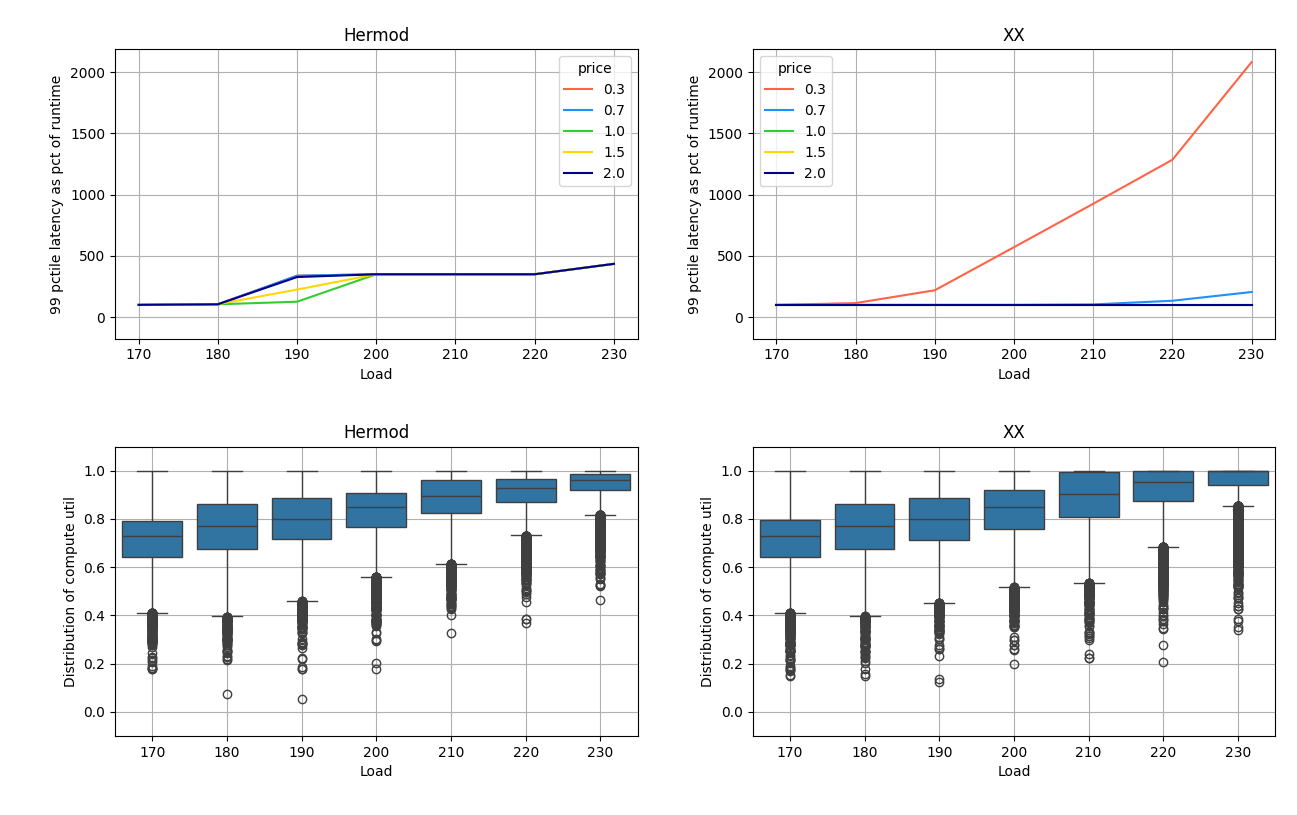
\includegraphics[width=8.5cm]{img/hermod_xx_latencies.png}
      \caption{ tail latency distribution and compute utilization across
      different loads, for Hermod and \sys{} }
    \label{fig:hermod-xx-edf}
\end{figure}


\subsection{Experimental Setup}

In each version of the simulator, functions arrive in an open loop at a constant
rate. The simulator attaches three main characteristics to each function it
generates: runtime, \priceclass{}, and memory usage.\ \textit{Function runtime}
is chosen by sampling from randomly generated long tailed (in this case pareto)
distribution: the relative length of the tail ($\alpha$ value) remains constant,
and the minimum value ($x_m$) is chosen from a normal distribution. This process
for sampling reflects the fact that different functions have different expected
runtimes (chosen from a normal distribution), and that actual invocation
runtimes follow long tailed distributions (so each pareto distribution that we
sample represents the expected runtime distribution of a given function).\
\textit{Function \class{}} is chosen randomly, but weighted: the simulator uses
a bimodal weighting across priorties. The simulator has $n$ different
\priceclass{} values, each assigned to a fictitious price. Because functions are
randomly assigned a \class{}, runtime and \class{} are not correlated.\
\textit{Function memory usage} is chosen randomly between 100MB and 10GB. Over
their lifetime, functions increase their memory usage from an initial amount
(always 100MB) to their total usage.

When comparing two different simulated schedulers, they each are given an
identical workload and then each simulate running that workload.

The simulator makes some simplifying assumptions:
\begin{enumerate}
    \item functions are compute bound, and do not block for i/o
    \item communication latencies are not simulated
    \item the amount of time it takes to swap memory is not simulated
\end{enumerate}

We simulate running 100 machines with 8 cores each, 4 scheduler shards, and a
k-choices value of 3 when applicable.

\subsection{How do function latencies compare?}

Developers care about function latency, so it is important to understand how
well \priceclass{}es do at reflecting and enforcing SLAs. On one hand, is
relevant to understand if we need \class{}es at all: is there a scheduler that
can, without having any access to information about which functions are latency
sensitive, still ensure that functions perform well? On the other hand, it is
helpful to compare \sys{} to an ideal scheduler, in order to contextualize
\sys{}'s performance.

To explore the first side of this question, we look at the performance of an
existing scheduler that does not take priority into account. We simulate
Hermod\cite{hermod}, a state-of-the-art research scheduler built specifically
for serverless. Hermod's design is the result of a from-first-principles
analysis of different scheduling paradigms. In accordance with the paper's
findings, we simulate least-loaded load balancing over machines found using
power-of-k-choices, combined with early binding and Processor Sharing
machine-level scheduling. Hermod does not use priorities in its design, and as
such the simulator ignores functions' \class{} when simulating Hermod's design.


On the other side, we want to simulate an ideal scheduler. Ideal is with respect
to meeting functions' SLAs, which requires defining the desired SLA. In order to
do this, we assign each function invocation a deadline, which we define as a
function of the true runtime as well as the \priceclass{}: deadline = runtime *
maxPrice/price. This definition ensures that the highest \class{}es functions'
deadlines are simply their runtimes, and deadlines get more and more slack with
lower \class{}es. We then simulate an Earliest Deadline First (EDF) scheduler
over these deadlines, which is queuing theoretically proven to be optimal in
exactly the way we wanted: if it is possible to create a schedule where all
functions meet their deadline, EDF will find it\cite{wiki-edf}. We run EDF in a
centralized setting: it schedules one machine with 800 cores, not 100 machines
with 8 each.

We compare the latencies observed in both of these settings with those that
running \sys{} produces. Because Hermod does not deal with memory pressure, and
to avoid an unfair comaprison with \sys{}'s swapping, we set the memory to be
absurdly high for all three settings in this experiment. We also turn off the
use of the idle list in \sys{}, so as to be on par with Hermod in placing load,
and revert solely to k-choices.

A strong result for \sys{} would show that it is able to maintain low latency
for high \priceclass{} functions. Especially under high load, we expect that the
differences betweeen the three approaches will become evident.
Figure~\ref{fig:hermod-xx-edf} shows the results. We can see that \sys{} and EDF
are able to retain performance for the high \class{} functions even under higher
load. EDF's superior performance on the far right side of the graph for the low
\class{} functions is because EDF runs only functions with short runtimes; the
others never finish and so don't show up on this graph. EDF's utilization is
also much tighter because of the centralised setting it runs in (so the spread
of the utilization comes from being different at different points in time, not
on different machines).


\subsection{Does \sys{} plan for memory management work?}

\begin{figure}[t!]
    \centering
      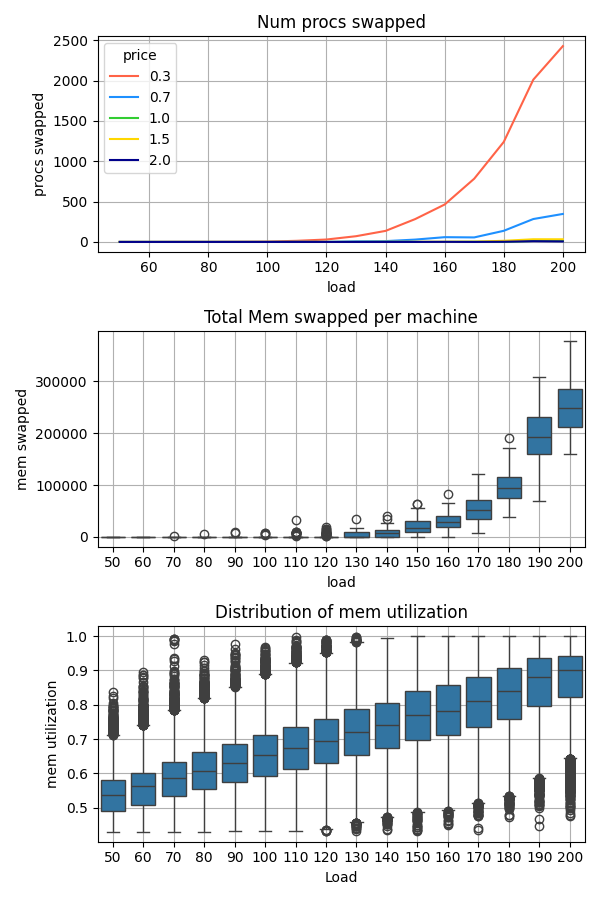
\includegraphics[width=8cm]{img/memory_graphs.png}
      \caption{ \sys{}'s swapping behavior. The amount of memory is in MB  }
    \label{fig:memory-graphs}
\end{figure}

To answer this question, we look at how \sys{} distributes load, and whether the
amount that \sys{} needs to swap memory is realistic. We now run \sys{} in a
setting of limited memory (32GB of RAM per machine), and track the memory
utilization of different machines, as well as how much and what machines need to
swap. A good result would show: a small spread of memory utilization, that
machines only start swapping once memory utilization is high, and that the
amount of swapping being done is equally spread across machines.
Figure~\ref{fig:memory-graphs} shows the results. We can see \sys{} swaps only
lower \class{} functions' memory, and that the amount of memory swapped is faily
evenly distributed between all the machines. We can also conclude that with a
500GB SSD, a provider would comfortably be able to avoid killing while running
the datacenter at an average memory utilization of $\sim$90$\%$, at the cost of
$\sim\$$30 per machine for swap space~\cite{ssd-price}.


